	% Kopfzeile beim Kapitelanfang:
\fancypagestyle{plain}{
%Kopfzeile links bzw. innen
\fancyhead[L]{\Large Vorlesung 15 (02.12.2013)}
%Kopfzeile rechts bzw. außen
\fancyhead[R]{}}
%Kopfzeile links bzw. innen
\fancyhead[L]{\Large Vorlesung 15 (02.12.2013)}
%Kopfzeile rechts bzw. außen
\fancyhead[R]{}
% **************************************************
\phantomsection
\addcontentsline{toc}{section}{\texorpdfstring{Graph der e-Funktion auf $\R$}{Graph der e-Funktion auf R}}
\section*{Graph der $e$-Funktion auf $\R$}
\begin{tikzpicture} [domain=-3:3]
\draw[->] (-3,0)--(3,0) node[right] {$x$};
\draw[->] (0,-0.5)--(0,3) node[above] {$f(x)$};
\draw[blue, domain=-3:1.2] plot (\x, {exp(\x)});
\draw[dashed] (1,0)--(1,2.7182818);
\draw[dashed] (0,2.7182818)--(1,2.7182818);
\draw (0,2.7182818) node{$-$} [left] node{$e$};
\draw (0,1) node{$-$} [left] node{$1$};
\draw (-0.3,-0.3) node{$0$};
\draw (1,0) node{$|$} [below] node{$1$};
\end{tikzpicture}

\phantomsection
\addcontentsline{toc}{section}{\texorpdfstring{Berechnung von $e^x$}{Berechnung von e hoch x}}
\section*{Berechnung von $e^x$}
$x \in \R \Ra x = g+x', x' \in [0,1), g \in \Z$\\
$\Ra e^x = e^g \cdot e^{x'}$\\
Bestimme also $e^x$ für $0 \le x < 1$\\
$e^x = \sum_{k=0}^\infty \frac{x^k}{k!} = \sum_{k=0}^n \frac{x^k}{k!} + R_{n+1}(x)$\\
$R_{n+1}(x)=\sum_{k=n+1}^\infty \frac{x^k}{k!}$ Restglied\\
$|x| \le 1 \Ra |R_{n+1}(x)| \underset{\vartriangle\text{-Ungl.}}{\le} \sum_{k=n+1}^\infty \frac{|x|^k}{k!} = \frac{|x|^{n+1}}{(n+1)!} \left(1+\frac{|x|}{n+2} + \frac{|x|^2}{(n+2)(n+3)} + \ldots\right)$\\
%$\le \frac{|x|^{n+1}}{(n+1)!} \left(1+\frac{|x|}{2} + \frac{|x|^2}{2 \cdot 2} + \ldots\right)$\\ %steht so nicht im Skriptum
$\le \frac{|x|^{n+1}}{(n+1)!} \left(\underbrace{1+\frac{1}{2}+\frac{1}{2^2}+\frac{1}{2^3}+\ldots}_{=2 \text{ (geom. Reihe)}}\right)$\\ %= \frac{2|x|^{n+1}}{(n+1)!}$\\ steht so nicht im Skriptum
Dabei gilt sogar striktes "`$<$"' statt "`$\le$"', falls $x \neq 0$.\\
Dieselbe Abschätzung funktioniert für $x \in \C$ mit $|x| \le 1$, also: %\\
%$e^x = 1 + x + \frac{x^2}{2} + \frac{x^3}{3!} + \ldots$ steht so nicht im Skriptum

\section{Satz: Restgliedabschätzung für die Exponentialfunktion}\label{8.12}
$x \in \C, |x| \le 1 \Ra e^x = \sum_{k=0}^n \frac{x^k}{k!} + R_{n+1}(x)$, wobei $|R_{n+1}(x)| \le 2 \cdot \underbrace{\frac{|x|^{n+1}}{(n+1)!}}_{\text{(*)}}$\\
dabei gilt ``$<$'', falls $x \neq 0$.\\
(*): Betrag des ersten weggelassenen Gliedes\nl
Speziell: $|x| \le 1 \Ra |e^x-1| \le 2|x|, |e^x-1-x| \le |x|^2$

\subsection*{Beispiel}
$e = e^1 = \sum_{k=0}^n \frac{1}{k!} + R_{n+1}(1), |R_{n+1}(1)| < \frac{2}{(n+1)!}$\\
$R_n(1) < 6 \cdot 10^{-8} \Ra e \approx 2,7182818$\\
Die exp. Reihe konvergiert rasch!

\section{Korollar}\label{8.13}
$e$ ist irrational.

\subsection*{Beweis}
Angenommen, $e=\frac{m}{n} \in \Q, m,n \in \N \Ra$\\
$s := \underbrace{\left(e - \sum_{k=0}^n \frac{1}{k!}\right)}_{\text{(*)}} n! \in \N$\nl
Aber: (*) $= R_{n+1}(1) \Ra s < n! \cdot \frac{2}{(n+1)!} \Ra s < \frac{2}{n+1}$ \wspruch

\subsection*{Bemerkung}
$e$ ist sogar \underline{transzendent}, das heißt $\nexists$ Polynom $p \in \Pow_{\R}$ mit \underline{rationalen} Koeffizienten, so dass $p(e)=0$.


\section{\texorpdfstring{Bemerkung: Weitere wichtige Darstellungen von $e^x$}{Bemerkung: Weitere wichtige Darstellungen von e hoch x}}\label{8.14}
$e^x = \lim_{n \to \infty} \left(1+\frac{x}{n}\right)^n, x \in \R$

\subsection*{Beweis}
Später.

\phantomsection
\addcontentsline{toc}{section}{Anwendung: Kontinuierliche Verzinsung}
\section*{Anwendung: Kontinuierliche Verzinsung}
Gegeben: Anfangskapital $K$, Zinssatz für ein Jahr: $p\%$ (Zinsfuß)\nl
Verzinsung: In jedem $\frac{1}{n}$-ten Jahr $\frac{p}{n}\%$ Zinsen auf das jeweils aktuelle Kapital\\
Kapital nach einem Jahr: $K \cdot \left(1 + \frac{p}{n} \cdot \frac{1}{100}\right)^n \underset{n \to \infty}{\to} K \cdot e^{\frac{p}{100}}$

\newpage

\phantomsection
\addcontentsline{toc}{section}{Sinus und Cosinus}
\section*{Sinus und Cosinus}\label{SinCos}

\subsection*{Vorüberlegung}
$z \in \C \to \overline{e^z} = e^{\overline{z}}$\\
Denn: $e^{\overline{z}} = \sum_{k=0}^\infty \frac{\overline{z}^k}{k!} = \lim_{n \to \infty} \sum_{k=0}^n \frac{\overline{z}^k}{k!} = \lim_{n \to \infty} \overline{\sum_{k=0}^n \frac{z^k}{k!}} \underset{\text{Regeln f. GW}}{=} \overline{\lim_{n \to \infty} \sum_{k=0}^n \frac{z^k}{k!}}$

\subsection*{Speziell}
$z = ix, x \in \R \Ra \overline{e^{ix}} = e^{\overline{ix}} = e^{-ix}$\\
$\Ra |e^{ix}|^2 = e^{ix} \cdot e^{-ix} \underset{\text{FG}}{=} e^0 = 1$\nl
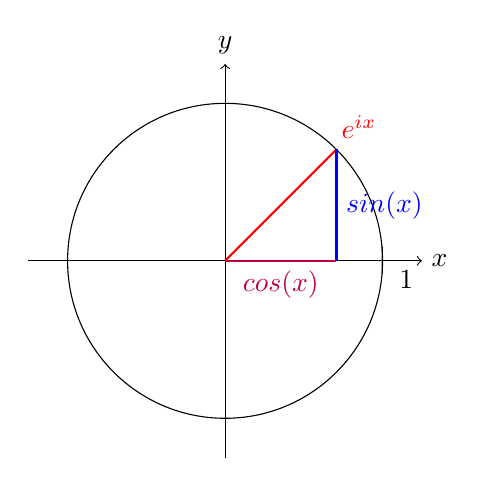
\begin{tikzpicture}
\draw[->] (-2.5,0)--(2.5,0) node[right] {$x$};
\draw[->] (0,-2.5)--(0,2.5) node[above] {$y$};
\draw (0,0) circle(2);
\draw[thick,color=red] (0,0)--(1.4142,1.4142);
\draw[color=red] (1.7,1.7) node {$e^{ix}$};
\draw[thick,color=blue] (1.4142,0)--(1.4142,1.4142);
\draw[color=blue] (1.4142,0.7071) node[right] {$sin(x)$};
\draw[thick,color=purple] (0,0)--(1.4142,0);
\draw[color=purple] (0.7071,0) node[below] {$cos(x)$};
\draw (2,0) node{$|$};
\draw (2.3,0) node[below]{$1$};
\end{tikzpicture}

\section{\texorpdfstring{Definition: Cosinus/Sinus auf $\R$}{Definition: Cosinus/Sinus auf \R}}\label{8.15}
\fbox{$\begin{array}{l} \cos x := \RE(e^{ix}) = \frac{1}{2} \cdot (e^{ix}+e^{-ix}) \nl \sin x := \IM(e^{ix}) = \frac{1}{2i} \cdot (e^{ix}-e^{-ix})\end{array}$}\nl
Damit folgt:

\section{Satz: Eulersche Formel}\label{8.16}
$x \in \R \Ra$ \fbox{$e^{ix}=\cos x + i \cdot \sin x$} \underline{Eulersche Formel}

\section{Satz}\label{8.17}
\en{
\item $cos^2 x + sin^2 x = 1$ [$cos^2 x = (cos \ x)^2$ etc.]\\
Insbes.: $-1 \le \cos x, sin \ x \le 1$
\item $cos(-x) = cos \ x$; $cos$ ist gerade; $cos \ 0 = 1$\\
$sin(-x) = -sin \ x$; $sin$ ist ungerade; $sin \ 0 = 0$
\item \underline{Additionstheoreme}:\\
$cos(x+y)=cos \ x \ cos \ y - sin \ x \ sin \ y$\\
$sin(x+y)=sin \ x \ cos \ y + cos \ x \ sin \ y$
}

\newpage

\subsection*{Beweis}
\en{
\item $cos^2 x + sin^2 x = [\RE(e^{ix})]^2 + [\IM(e^{ix})]^2 = |e^{ix}|^2 = 1$
\item klar aus Definition
\item $e^{i(x+y)} \underset{\text{FG}}{=} e^{ix} \cdot e^{iy} \Ra cos(x+y) + i \cdot sin(x+y) = (cos \ x + i \cdot sin \ x) \cdot (cos \ y + i \cdot sin \ y)$\\
$= cos \ x \ cos \ y - sin \ x \ sin \ y + i(cos \ x \ sin \ y + sin \ x \ cos \ y)$
}
Vergleich der Real-/Imaginärteile $\Ra$ Behauptung. \qed

\section{Satz: Reihenentwicklung des Sinus/Cosinus}\label{8.18}
$\forall x \in \R$ gilt:
\en{
\item $cos \ x = \sum_{k=0}^\infty (-1)^k \cdot \frac{x^{2k}}{(2k)!} = 1 - \frac{x^2}{2} + \frac{x^4}{24} - \frac{x^6}{6!} \pm \ldots$
\item $sin \ x = \sum_{k=0}^\infty (-1)^k \cdot \frac{x^{2k+1}}{(2k+1)!} = x - \frac{x^3}{6} + \frac{x^5}{5!} \mp \ldots$
}
Beide Reihen sind absolut konvergent.

\subsection*{Beweis}
Für Cosinus:\\
$cos \ x = \frac{1}{2} (e^{ix} + e^{-ix}) = \frac{1}{2}\left(\sum_{k=0}^\infty \frac{(ix)^k}{k!} + \sum_{k=0}^\infty \frac{(-ix)^k}{k!}\right)$\\
$=\frac{1}{2} \sum_{k=0}^\infty (1+(-1)^k) \frac{(ix)^k}{k!}$\\
$=\sum_{\underset{k \text{ gerade}}{k=0}}^\infty \frac{(ix)^k}{k!} \underset{(k=2n)}{=} \sum_{n=0}^\infty \frac{(-1)^n x^{2n}}{(2n)!}$\nl
Analog für den Sinus.\\
Die Reihen für $e^{ix}, e^{-ix}$ konvergieren absolut\\
$\Ra$ die Cosinus- und Sinus-Reihen konvergieren absolut, wegen dem

\section{Lemma}\label{8.19}
Seien $\sum_{k=0}^\infty z_k, \sum_{k=0}^\infty w_k$ absolut konvergent ($z_k, w_k \in \C$)\\
$\Ra \sum_{k=0}^\infty (z_k+w_k), \sum_{k=0}^\infty \overline{z_k}$ sind absolut konvergent.

\subsection*{Beweis}
$\sum_{k=0}^\infty (|z_k|+|w_k|)$ bzw. $\sum_{k=0}^\infty |z_k|$ sind konvergente Majoranten. \qed

\subsection*{Später}\label{SinCosGraph}
$cos$ und $sin$ sind $2 \pi$-periodisch, $\frac{\pi}{2} :=$ erste positive Nullstelle von $cos$\nl
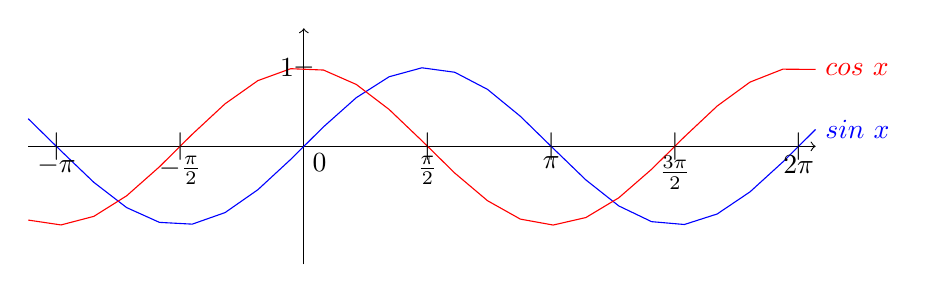
\begin{tikzpicture}
\draw[->] (-3.5,0)--(6.5,0);
\draw[->] (0,-1.5)--(0,1.5);
\draw[blue, domain=-3.5:6.5] plot (\x, {sin(deg(\x))}) node[right] {$sin \ x$};
\draw[red, domain=-3.5:6.5] plot (\x, {cos(deg(\x))}) node[right] {$cos \ x$};
\draw (0,1) node{$-$} [left] node{$1$};
\draw (0.2,-0.2) node{$0$};
\draw (-3.1415927,0) node{$|$} [below] node{$-\pi$};
\draw (-1.5707963,0) node{$|$} [below] node{$-\frac{\pi}{2}$};
\draw (1.5707963,0) node{$|$} [below] node{$\frac{\pi}{2}$};
\draw (3.1415927,0) node{$|$} [below] node{$\pi$};
\draw (4.712389,0) node{$|$} [below] node{$\frac{3\pi}{2}$};
\draw (6.2831853,0) node{$|$} [below] node{$2\pi$};
\end{tikzpicture}

\section{Einschließungslemma}\label{8.20}
Für $x \in [0,2]$ gilt:
\en{
\item ${\color{blue} 1 - \frac{x^2}{2}} \le cos \ x \le {\color{red} 1 - \frac{x^2}{2} + \frac{x^4}{24}}$
\item $0 \le {\color{blue} x - \frac{x^3}{6}} \le sin \ x \le {\color{red} x}$
}
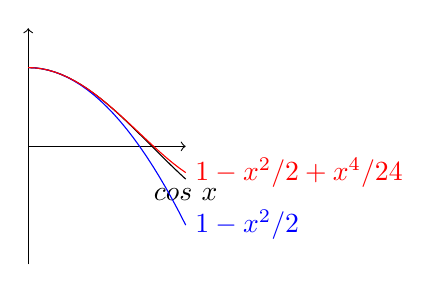
\begin{tikzpicture}
\draw[->] (0,0)--(2,0);
\draw[->] (0,-1.5)--(0,1.5);
\draw[domain=0:2] plot (\x, {cos(deg(\x))}) node[below] {$cos \ x$};
\draw[blue, domain=0:2] plot (\x, {1-(\x^2/2)}) node[right] {$1-x^2/2$};
\draw[red, domain=0:2] plot (\x, {1-(\x^2/2)+(\x^4/24)}) node[right] {$1-x^2/2+x^4/24$};
\end{tikzpicture} \ 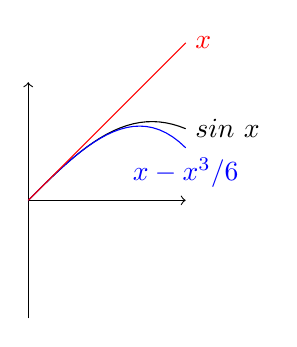
\begin{tikzpicture}
\draw[->] (0,0)--(2,0);
\draw[->] (0,-1.5)--(0,1.5);
\draw[domain=0:2] plot (\x, {sin(deg(\x))}) node[right] {$sin \ x$};
\draw[blue, domain=0:2] plot (\x, {\x-(\x^3/6)}) node[below] {$x-x^3/6$};
\draw[red, domain=0:2] plot (\x, {\x}) node[right] {$x$};
\end{tikzpicture}

\subsection*{Beweis}
\en{
\item $cos \ 0 = 1 \Ra$ richtig für $x = 0$\\
$0 < x \le 2 \Ra cos \ x = \sum_{k=0}^\infty (-1)^k \underbrace{\frac{x^{2k}}{(2k)!}}_{a_k > 0}$ alternierend\\
$\frac{a_{k+1}}{a_k} = \frac{x^2}{(2k+2)(2k+1)} \le \frac{4}{(2k+2)(2k+1)} < 1$ für $k \ge 1$\\
$\Ra (a_k)_{k \ge 1}$ monoton fallende Nullfolge (nächstes Mal)
}